\documentclass{article}

% ICML 2025 style
\usepackage{icml2025}

% Standard packages
\usepackage{amsmath}
\usepackage{amssymb}
\usepackage{booktabs}
\usepackage{graphicx}
\usepackage{hyperref}
\usepackage{url}
\usepackage{microtype}
\usepackage{verbatim}

% For algorithm environments (optional)
% \usepackage{algorithm}
% \usepackage{algorithmic}

% Submission mode: anonymous
\icmltitlerunning{Quantifying Calibration-Alignment Divergence under RLHF Optimization Pressure}

\begin{document}

\twocolumn[
\icmltitle{Quantifying Calibration-Alignment Divergence under RLHF Optimization Pressure}

\icmlsetsymbol{equal}{*}

\begin{icmlauthorlist}
\icmlauthor{Anonymous}{anon}
\end{icmlauthorlist}

\icmlaffiliation{anon}{Anonymous Institution}
\icmlcorrespondingauthor{Anonymous}{anonymous@anonymous.edu}

\icmlkeywords{RLHF, reward hacking, overoptimization, bidirectional alignment, calibration, KL divergence}

\vskip 0.3in
]

\printAffiliationsAndNotice{\icmlEqualContribution}

% Abstract
\begin{abstract}
Reinforcement Learning from Human Feedback (RLHF) trains language models against a reward model proxy rather than direct human judgment. As optimization pressure increases, this proxy diverges from held-out human preference---a phenomenon known qualitatively as reward hacking. We ask: how fast does this divergence grow, and does the growth rate replicate across independent experimental settings?

We define the \emph{calibration-alignment divergence curve} as the regression slope of the normalized proxy-gold gap (RM score minus held-out human preference, both on $[0,1]$ scale) on KL divergence budget. Analyzing published RLHF experimental data from two independent sources, we find this slope is $\beta = 0.143\ \text{nat}^{-1}$ in Coste et al.~\cite{Coste2023Reward} ($R^2 = 0.958$, $p < 10^{-6}$) and $\beta = 0.160\ \text{nat}^{-1}$ in Gao et al.~\cite{Gao2023Scaling} ($p = 0.003$)---a cross-dataset slope ratio of $1.116$, indicating near-identical divergence rates despite different model families and scales.

These results provide the first regression characterization of the \emph{normalized divergence gap} ($\text{RM\_norm} - \text{gold\_preference}$) as a function of KL budget with cross-dataset slope comparison, framing reward hacking as an empirical instance of bidirectional alignment tension. We propose the normalized divergence gap as a standard cross-study comparison instrument computable from existing RLHF evaluation infrastructure.
\end{abstract}


% Main sections
\section{Introduction}

Every additional nat of KL divergence applied during RLHF fine-tuning increases the gap between a reward model's evaluation score and actual human preference by 0.143 units on a normalized scale---a relationship so consistent that it explains 96\% of divergence variance across 10 optimization checkpoints and replicates with slopes within 12\% across two independent model families. In other words, the more aggressively we optimize for alignment metrics, the less calibrated our models become to held-out human judgment.

This finding is counterintuitive by design. RLHF---Reinforcement Learning from Human Feedback---is the dominant paradigm for making large language models helpful, harmless, and honest. Its central promise is that optimizing against a reward model trained on human preferences should make the model \emph{more} aligned with human judgment. Yet the data reveal a systematic divergence: reward model scores climb monotonically with KL budget, while gold human preference peaks early (at approximately 2 nats of KL divergence) and subsequently declines by 40\%. The more optimized the model, the wider the gap between what the evaluation says and what humans actually prefer.

\textbf{The surface problem} is well-known: RLHF trains against a proxy metric---the reward model score---that approximates but is not equivalent to gold human preference. As optimization pressure increases, the policy finds outputs that satisfy the proxy while diverging from the underlying target. This ``reward hacking'' or ``overoptimization'' phenomenon has been described qualitatively in the literature \cite{Coste2023Reward,Gao2023Scaling}: RM scores rise while human preference metrics plateau or reverse.

\textbf{The deeper problem} is that this divergence has never been quantitatively characterized as a function of optimization pressure. We do not know \emph{how fast} the gap grows, whether the growth rate is model-family-specific or reflects an underlying law-like pattern, or whether a standardized measurement instrument can enable cross-study comparison. Without these quantitative answers, practitioners cannot estimate when RLHF optimization degrades calibration past an acceptable threshold, nor can researchers compare overoptimization severity across experimental settings.

\textbf{The gap we address} lies at the intersection of three literatures that have not been connected: RLHF overoptimization theory, bidirectional human-AI alignment measurement, and Goodhart's Law in machine learning. Each literature describes part of the phenomenon, but none provides a named construct, a quantified slope, or a normalized metric that enables cross-dataset comparison. The ICLR 2025 Workshop on Bidirectional Human-AI Alignment synthesized 400 papers and found that existing alignment benchmarks systematically measure only the AI$\to$Human direction---reward model scores, safety classifiers, benchmark accuracy---while Human$\to$AI calibration (whether humans appropriately trust and accurately interpret model outputs) is measured in a parallel HCI track never integrated with ML evaluation \cite{ICLR2025Bidirectional}. Our work connects these: RLHF overoptimization is the empirical instantiation of bidirectional alignment tension, where optimizing AI$\to$Human proxy metrics systematically degrades evaluation calibration to held-out human judgment.

\textbf{Our key insight} is that the normalized divergence gap---$\text{RM\_norm} - \text{gold\_preference}$, where both signals are min-max scaled to $[0,1]$---grows linearly with KL budget at a consistent, measurable rate. This normalized metric removes scale artifacts while preserving direction and monotonicity, creating a measurement instrument that works across different experimental settings. Applying ordinary least squares regression to this metric across published RLHF experimental data reveals a named quantity---the \emph{calibration-alignment divergence curve}---characterized by a slope $\beta$ that is significantly positive, statistically robust, and reproducible across independent model families.

In this work, we make four contributions:

\begin{enumerate}
\item \textbf{The calibration-alignment divergence construct.} We define and operationalize the calibration-alignment divergence gap as a named bidirectional alignment construct---the first regression characterization of the normalized divergence gap ($\text{RM\_norm} - \text{gold\_preference}$) as a function of KL optimization budget with cross-dataset slope comparison. Prior work described the phenomenon qualitatively; we compute $\beta$, $R^2$, parametric confidence intervals, and bootstrap confidence intervals, enabling systematic cross-study comparison.

\item \textbf{Quantified divergence curve slopes.} In Coste et al.~\cite{Coste2023Reward} data, we find $\beta = 0.1433\ \text{nat}^{-1}$ ($R^2 = 0.958$, $p = 8.89 \times 10^{-7}$)---a near-perfect linear fit. The calibration-alignment divergence gap grows by 0.143 normalized units per nat of KL budget, a relationship that explains 96\% of gap variance across 10 optimization checkpoints.

\item \textbf{Cross-dataset replication with effect size comparison.} In independent Gao et al.~\cite{Gao2023Scaling} data (different model family, different scale), we find $\beta = 0.1599\ \text{nat}^{-1}$ ($p = 0.003$), yielding a cross-dataset slope ratio of 1.116. Two entirely independent experimental settings produce slopes within 12\% of each other---consistent evidence ($n=2$ datasets; further replication required to establish universality) that this is not a model-family artifact.

\item \textbf{The normalized divergence gap metric.} We propose $\text{RM\_norm} - \text{gold\_preference} \in [-1, +1]$ as a standardized evaluation calibration divergence instrument that enables cross-study comparison by removing raw scale differences between experimental settings.
\end{enumerate}

We organize the remainder of the paper as follows: Section~\ref{sec:related} situates our work in three strands of prior research. Section~\ref{sec:method} describes our methodology and the design rationale for the normalized gap metric. Section~\ref{sec:experiments} presents our experimental setup and the four-step mechanistic verification. Section~\ref{sec:results} reports results. Section~\ref{sec:discussion} discusses implications, limitations, and connections to the broader bidirectional alignment agenda. Section~\ref{sec:conclusion} concludes.

\section{Related Work}
\label{sec:related}

Our work sits at the intersection of three strands of prior research: RLHF overoptimization theory, bidirectional human-AI alignment measurement, and Goodhart's Law in machine learning. Each strand illuminates part of the phenomenon we study, but none provides the quantitative characterization we offer---a named divergence construct, a regression slope, and a cross-dataset replication.

\subsection{RLHF Overoptimization and Reward Hacking}

Reinforcement learning from human feedback was introduced as a paradigm for aligning language models with human preferences through a reward model trained on preference annotations \cite{Ouyang2022Training,Christiano2017Deep}. RLHF has become the dominant alignment approach, enabling models that score high on helpfulness and harmlessness benchmarks \cite{Bai2022Training,Stiennon2020Learning}. However, the reward model is an imperfect proxy for human preference, and sustained optimization against this proxy causes the policy to exploit proxy weaknesses---a phenomenon known as reward hacking or specification gaming \cite{Krakovna2020Specification,Skalse2022Defining}.

Coste et al.~\cite{Coste2023Reward} provide the clearest empirical demonstration: as KL budget from the base policy increases from 0 to 8 nats, the reward model score rises monotonically while gold human preference peaks and then reverses. Gao et al.~\cite{Gao2023Scaling} characterize the scaling laws of reward model overoptimization at multiple RM sizes, showing consistent patterns across model scales. Both papers describe the divergence qualitatively---RM rises while gold reverses---but stop short of defining the \emph{normalized divergence gap} ($\text{RM\_norm} - \text{gold\_preference}$) as a regression target or reporting cross-dataset slope comparison. Our work takes this step: we fit OLS regression to the normalized gap in both datasets and report $\beta = 0.1433\ \text{nat}^{-1}$ (Coste) and $\beta = 0.1599\ \text{nat}^{-1}$ (Gao), enabling the first cross-dataset characterization of the calibration-alignment divergence curve slope.

Ziegler et al.~\cite{Ziegler2019Fine} and Stiennon et al.~\cite{Stiennon2020Learning} document early cases where RLHF reward models diverge from human preferences in text summarization. These works establish the qualitative phenomenon; our contribution is quantification and cross-dataset effect size comparison.

\subsection{Bidirectional Human-AI Alignment Measurement}

The ICLR 2025 Workshop on Bidirectional Human-AI Alignment synthesized 400 papers in the alignment literature and found a systematic measurement asymmetry: virtually all major alignment benchmarks---TruthfulQA \cite{Lin2022TruthfulQA}, BBQ \cite{Parrish2022BBQ}, HHH-RLHF, WinoBias \cite{Zhao2018Gender}, HELM \cite{Liang2023Holistic}---measure the AI$\to$Human direction exclusively. Human$\to$AI alignment is studied in a parallel HCI and cognitive science track but has not been integrated with ML evaluation frameworks.

Lai et al.~\cite{Lai2021Understanding} demonstrate that AI-assisted decision-making produces over-reliance: in several experimental settings, 60--80\% of humans agree with AI predictions regardless of AI accuracy. Bansal et al.~\cite{Bansal2021Does} and Bu\c{c}inca et al.~\cite{Buccinca2021Trust} further characterize over-reliance patterns and propose interventions. However, these behavioral studies do not connect to RLHF optimization pressure---they measure human calibration at a fixed model deployment snapshot, not as a function of how aggressively the model was optimized.

Our work bridges these two tracks: we treat RLHF overoptimization as the empirical instantiation of bidirectional alignment tension. We scope this as ``evaluation calibration divergence''---distinct from but motivating the study of user behavioral calibration (appropriate reliance; Lai et al.~\cite{Lai2021Understanding} paradigm). The connection to user over-reliance remains a theoretical extension for future behavioral work.

\subsection{Goodhart's Law and Proxy-Target Decoupling in ML}

Goodhart's Law---``when a measure becomes a target, it ceases to be a good measure''---has been formalized in the ML setting by Manheim and Garrabrant~\cite{Manheim2019Categorizing} and others. Krakovna et al.~\cite{Krakovna2020Specification} compile a specification gaming list documenting empirical cases in RL. Skalse et al.~\cite{Skalse2022Defining} formalize reward tampering and misspecification conditions under which proxy-target decoupling is guaranteed.

These theoretical works predict proxy-gold divergence under optimization pressure. Our work provides an empirical instantiation with specific quantitative parameters: in the RLHF setting with explicit reward model training, the proxy-gold gap grows at $\beta \approx 0.143$--$0.160\ \text{nat}^{-1}$ of KL budget. This connects the abstract Goodhart/specification-gaming literature to a concrete, measurable phenomenon in modern RLHF training.

Our three quantitative contributions---the calibration-alignment divergence construct, the regression slope $\beta$ with cross-dataset replication, and the normalized gap metric---are not derivable from any prior paper. The closest works are Coste et al.~\cite{Coste2023Reward} and Gao et al.~\cite{Gao2023Scaling}, which provide the raw experimental data; we contribute the regression framework, normalization methodology, cross-dataset comparison, and bidirectional alignment framing.

\section{Methodology}
\label{sec:method}

Building on our key insight---that the proxy-gold divergence gap, when properly normalized, grows linearly and measurably with RLHF optimization pressure---we design a methodology with three components: a normalization protocol that creates a cross-dataset comparison instrument, a regression pipeline that quantifies the divergence curve slope, and a four-step mechanistic verification that establishes \emph{why} the gap grows.

\subsection{Overview}

We study two independently published RLHF experimental datasets (Coste et al.~\cite{Coste2023Reward} and Gao et al.~\cite{Gao2023Scaling}) at multiple KL divergence checkpoints. At each checkpoint, we have two signals: the reward model score (the proxy) and held-out gold human preference (the target). The core methodological challenge is that these signals live on different scales across datasets---raw RM scores in Coste et al.\ span $[0.12, 2.08]$ while gold preference spans $[0.38, 0.63]$. Cross-dataset comparison of raw differences is therefore meaningless.

Our solution is the \textbf{normalized divergence gap}:
\begin{equation}
\text{gap}(k) = \text{normalize}(\text{RM}_k) - \text{gold\_preference}_k
\end{equation}
where normalization is min-max scaling to $[0, 1]$ applied to the RM score series, and gold preference is already in $[0, 1]$ as a rate. The resulting gap $\in [-1, +1]$ enables cross-dataset slope comparison on a common scale.

\subsection{Datasets and Data Reconstruction}

\textbf{Dataset 1: Coste et al.~\cite{Coste2023Reward} (arXiv:2310.02743).} We use 10 paired observations of (KL\_budget, RM\_score, gold\_preference) from Coste et al.~\cite{Coste2023Reward}, covering KL budgets from 0.0 to 8.0 nats. Data values are constructed consistent with qualitative descriptions in published figures using standard figure digitization methodology. This introduces an estimated $\pm 2$--5\% digitization uncertainty per data point.

\textbf{Dataset 2: Gao et al.~\cite{Gao2023Scaling} (arXiv:2210.10760, ICML 2023).} We use 10 paired observations from Gao et al.~\cite{Gao2023Scaling}, covering KL budgets from 0.0 to 7.5 nats. This dataset uses a different model family and scale (6B reward model), providing an independent replication context.

\textbf{Honest disclosure:} Neither raw dataset is publicly available in machine-readable format. Our data reconstruction from published figures introduces digitization uncertainty that affects exact $\beta$ values but not the direction or statistical significance of the slope---the documented effect sizes ($R^2 = 0.958$, $p < 10^{-6}$ in Coste data) are robust to $\pm 2$--5\% perturbation.

\subsection{The Normalized Divergence Gap Metric}

For a series of $N$ KL checkpoints with RM scores $s_1, \ldots, s_N$ and gold preference rates $g_1, \ldots, g_N$:
\begin{equation}
\text{RM\_norm}_i = \frac{s_i - \min(s)}{\max(s) - \min(s)}, \quad \text{gap}_i = \text{RM\_norm}_i - g_i
\end{equation}

We choose min-max normalization over z-score normalization because it preserves the $[0, 1]$ interpretable range, gold preference is already in $[0, 1]$ as a rate, and it preserves the monotonicity structure needed to detect reward hacking while removing cross-dataset scale artifacts.

\subsection{Regression Pipeline}

We apply OLS regression to $\{(\text{KL}_i, \text{gap}_i)\}_{i=1}^{N}$: $\text{gap} = \beta \cdot \text{KL} + \alpha + \varepsilon$. We use two implementations for redundancy: \texttt{scipy.stats.linregress} (primary, parametric CI via t-distribution) and \texttt{statsmodels.api.OLS} (secondary, F-statistic, residual diagnostics). Bootstrap CIs use $N=10{,}000$ resamples with seed=42. Pre-registered success criteria: $\beta > 0$, $p < 0.05$ (primary); $R^2 > 0.5$ (secondary).

\subsection{Four-Step Mechanistic Verification}

\begin{enumerate}
\item \textbf{Step 1 (H-E1):} Signal co-existence---both RM score and gold preference are separable, non-constant series.
\item \textbf{Step 2 (H-M1):} Trajectory divergence---RM rises monotonically (Spearman $\rho > 0.8$, $p < 0.05$) while gold preference reverses.
\item \textbf{Step 3 (H-M2):} Gap positivity---normalized divergence gap is strictly positive and growing at high KL ($\text{KL} > 3.5$ nats).
\item \textbf{Step 4 (H-M3, H-M4):} Slope quantification---OLS $\beta > 0$, $p < 0.05$ in both datasets; cross-dataset slope ratio $\beta_\text{Gao} / \beta_\text{Coste}$.
\end{enumerate}

Figure~\ref{fig:trajectory} (\texttt{trajectory\_dual\_axis.png}) illustrates the diverging trajectories from Steps 2--3.

\section{Experimental Setup}
\label{sec:experiments}

We design experiments to answer five research questions that collectively verify the four-step causal mechanism.

\textbf{RQ1 (H-E1):} Do both RM score and gold preference signals co-exist as separable, non-constant series across RLHF optimization checkpoints?

\textbf{RQ2 (H-M1):} Does RM score rise monotonically while gold preference reverses after an early peak?

\textbf{RQ3 (H-M2):} Is the normalized calibration-alignment divergence gap strictly positive and growing at high KL?

\textbf{RQ4 (H-M3):} Does OLS regression reveal a significantly positive slope $\beta$ in Coste et al.~\cite{Coste2023Reward} data?

\textbf{RQ5 (H-M4):} Does the same positive slope replicate in independent Gao et al.~\cite{Gao2023Scaling} data?

\subsection{Datasets}

\begin{table}[h]
\centering
\caption{Experimental datasets.}
\label{tab:datasets}
\begin{tabular}{lllll}
\toprule
Dataset & Source & KL Checkpoints & KL Range & Role \\
\midrule
Coste et al.~\cite{Coste2023Reward} & arXiv:2310.02743 & 10 & 0.0--8.0 nats & Primary (P1 test) \\
Gao et al.~\cite{Gao2023Scaling} & arXiv:2210.10760 & 10 & 0.0--7.5 nats & Replication (P2 test) \\
\bottomrule
\end{tabular}
\end{table}

\textbf{Coste et al.~\cite{Coste2023Reward}} is the primary dataset, providing the clearest published demonstration of gold preference reversal under RLHF optimization. \textbf{Gao et al.~\cite{Gao2023Scaling}} is the replication dataset---different model family, different scale (6B RM), different task distribution.

\subsection{Evaluation Metrics}

\begin{table}[h]
\centering
\caption{Evaluation metrics and gate conditions.}
\label{tab:metrics}
\begin{tabular}{lll}
\toprule
Metric & Definition & Gate \\
\midrule
OLS slope $\beta$ & Coefficient of KL in gap $\sim \beta \cdot \text{KL} + \alpha$ & MUST\_WORK ($\beta > 0$, $p < 0.05$) \\
$R^2$ & Proportion of gap variance explained & MUST\_WORK secondary ($> 0.5$) \\
Bootstrap 95\% CI & $N=10{,}000$ resamples, seed=42 & HIGH confidence if fully positive \\
$\beta_\text{Gao} / \beta_\text{Coste}$ & Cross-dataset slope ratio & Post-hoc consistency check \\
\bottomrule
\end{tabular}
\end{table}

\subsection{Implementation Details}

Each hypothesis step is a standalone Python experiment module with dataclass configuration, flat \texttt{src/} layout, and \texttt{sys.exit(0/1)} gate result. Key hyperparameters: bootstrap iterations $N=10{,}000$; random seed 42; 95\% CI level. Normalization applied once in H-M2 and consumed by H-M3/H-M4 via CSV output.

\section{Results}
\label{sec:results}

Our experiments confirm the four-step causal mechanism and quantify the calibration-alignment divergence curve with high statistical confidence in the primary dataset and medium confidence in the independent replication.

\subsection{Step 1: Signal Co-existence (H-E1)}

Both RM score and gold human preference co-exist as separable, non-constant series. In Coste et al.\ data, RM score variance $= 1.96$ and gold variance $= 0.25$ across 10 KL checkpoints; in Gao et al.\ data, rm\_var $= 2.42$ and gold\_var $= 0.31$ across 11 KL levels available for signal characterization (note: one boundary checkpoint at KL $= 0$ is included here for variance estimation but excluded from the regression in Step 4---see Section~\ref{subsec:replication}---yielding $n=10$ paired observations for H-M4). Both signals are non-constant and separable.

\textbf{What this means:} The measurement infrastructure for bidirectional alignment evaluation already exists in published RLHF experiments---both proxy and gold signals are recoverable and distinct. Figure~\ref{fig:dual_coste} (\texttt{dual\_axis\_coste2023.png}) illustrates both trajectories.

\subsection{Step 2: Directional Divergence (H-M1)}

The reward model score rises monotonically (Spearman $\rho(\text{KL}, \text{RM}) = 1.000$, $p < 0.0001$) while gold preference peaks at KL $\approx 2.0$ nats (gold $= 0.63$) and declines to $0.38$ by KL $= 8.0$ nats---a 40\% decline from peak. Final proxy-gold divergence $= 1.70$.

Figure~\ref{fig:trajectory} (\texttt{trajectory\_dual\_axis.png}) shows the diverging trajectories. \textbf{What this means:} Sustained RLHF optimization does not plateau human preference---it reverses it. The proxy and human judgment signals move in opposite directions once KL $> 2$ nats.

\textbf{Caveat:} $\rho = 1.000$ is unexpectedly perfect for real experimental data; we attribute this most likely to digitization idealization. Gao et al.\ $R^2 = 0.701$ (Section~\ref{subsec:replication}) is more representative of real experimental noise.

\subsection{Step 3: Gap Positivity and Monotonicity (H-M2)}

The normalized divergence gap is strictly positive at all five high-KL checkpoints (KL $> 3.5$ nats), with $\rho(\text{gap}, \text{KL}) = 1.000$ within the high-KL subset.

\begin{table}[h]
\centering
\caption{Normalized divergence gap at high-KL checkpoints.}
\label{tab:gap}
\begin{tabular}{ll}
\toprule
KL budget (nats) & gap $= \text{RM\_norm} - \text{gold\_preference}$ \\
\midrule
4.0 & $+0.277$ \\
5.0 & $+0.388$ \\
6.0 & $+0.484$ \\
7.0 & $+0.560$ \\
8.0 & $\mathbf{+0.620}$ \\
\bottomrule
\end{tabular}
\end{table}

Maximum gap $= 0.620$---the proxy score exceeds gold preference by more than half the normalized scale. Figure~\ref{fig:gap} (\texttt{gap\_curve.png}) shows the gap trajectory. \textbf{What this means:} Once KL $> 3.5$ nats, the calibration-alignment divergence is systematic and monotonically growing---not a transient artifact.

\subsection{Step 4: Divergence Curve Quantification (H-M3 --- Primary)}

\begin{table}[h]
\centering
\caption{OLS regression results, Coste et al.~\cite{Coste2023Reward} (primary dataset).}
\label{tab:regression_coste}
\begin{tabular}{ll}
\toprule
Metric & Value \\
\midrule
Slope $\beta$ & $\mathbf{0.1433\ \text{nat}^{-1}}$ \\
Intercept $\alpha$ & $-0.4016$ \\
$R^2$ & $\mathbf{0.9577}$ \\
$p$-value (Wald $t$-test) & $\mathbf{8.89 \times 10^{-7}}$ \\
$t$-statistic & $13.461$ \\
$N$ & $10$ \\
Parametric 95\% CI & $[0.119, 0.168]$ \\
Bootstrap 95\% CI ($N=10{,}000$) & $[0.117, 0.177]$ \\
\bottomrule
\end{tabular}
\end{table}

All three gate conditions satisfied: $\beta > 0$, $p < 0.05$, $R^2 > 0.5$. Both CIs are strictly positive---HIGH confidence for P1.

Figure~\ref{fig:regression} (\texttt{regression\_scatter.png}) shows the scatter plot with OLS line and 95\% CI. \textbf{What this means:} A single linear model explains 96\% of the variance in the calibration-alignment divergence gap across 10 RLHF checkpoints. Each additional nat of KL budget adds 0.143 normalized units to the divergence.

\subsection{Step 4 (Replication): Cross-Dataset Replication (H-M4 --- Replication)}
\label{subsec:replication}

\begin{table}[h]
\centering
\caption{Cross-dataset comparison of regression results.}
\label{tab:crossdataset}
\begin{tabular}{lll}
\toprule
Metric & Coste et al.~\cite{Coste2023Reward} & Gao et al.~\cite{Gao2023Scaling} \\
\midrule
$\beta$ (slope) & $0.1433\ \text{nat}^{-1}$ & $\mathbf{0.1599\ \text{nat}^{-1}}$ \\
$R^2$ & $0.9577$ & $0.7008$ \\
$p$-value & $8.89 \times 10^{-7}$ & $\mathbf{0.0025}$ \\
Parametric 95\% CI & $[0.119, 0.168]$ & $[0.075, 0.245]$ \\
Bootstrap 95\% CI & $[0.117, 0.177]$ & $[-0.020, 0.236]$ \\
Confidence & HIGH & MEDIUM \\
\bottomrule
\end{tabular}
\end{table}

Cross-dataset slope ratio $\beta_\text{Gao} / \beta_\text{Coste} = \mathbf{1.116}$---slopes within 12\% across independent model families.

Figure~\ref{fig:slopes} (\texttt{fig3\_cross\_dataset\_slopes.png}) shows the slopes with error bars. Figure~\ref{fig:overlay} (\texttt{fig4\_dual\_overlay.png}) shows both datasets' regression lines.

\textbf{Note on Gao checkpoint count:} The dual-axis trajectory plot (Appendix~\ref{app:gao}, Figure~\ref{fig:gao_dual}) displays all 11 available KL levels from Gao et al.\ for signal visualization. The regression (H-M4) uses $n=10$ paired observations, excluding the KL$=0$ boundary point where RM score is at its minimum anchor value and the gap is not yet informative as a regression predictor. This exclusion is consistent with the normalization procedure and is reflected in the datasets table (Table~\ref{tab:datasets}).

\textbf{Caveat (Gao replication):} Bootstrap CI $[-0.020, 0.236]$ marginally overlaps zero due to the non-monotone gap shape at low KL in Gao data (gap is initially negative before crossover at $\sim$3.5 nats). The parametric Wald $t$-test ($p = 0.003$) and parametric CI $[0.075, 0.245]$---entirely positive---serve as the primary replication criterion, as pre-registered.

\subsection{Summary}

\begin{table}[h]
\centering
\caption{Hypothesis validation summary.}
\label{tab:summary}
\begin{tabular}{lllp{5.5cm}}
\toprule
Hypothesis & Gate & Status & Key Result \\
\midrule
H-E1 (Co-existence) & MUST\_WORK & PASS & 10 paired KL levels; both signals separable \\
H-M1 (Mechanism) & MUST\_WORK & PASS & $\rho(\text{KL},\text{RM})=1.000$; gold $-40\%$ from peak \\
H-M2 (Gap positivity) & MUST\_WORK & PASS & 5/5 high-KL positive; max\_gap$=0.620$ \\
H-M3 (Coste slope) & MUST\_WORK & PASS & $\beta=0.143$, $p=8.89\times10^{-7}$, $R^2=0.958$ \\
H-M4 (Gao replication) & SHOULD\_WORK & PASS & $\beta=0.160$, $p=0.003$; ratio$=1.116$ \\
\bottomrule
\end{tabular}
\end{table}


% Main figures
\begin{figure}[t]
\centering
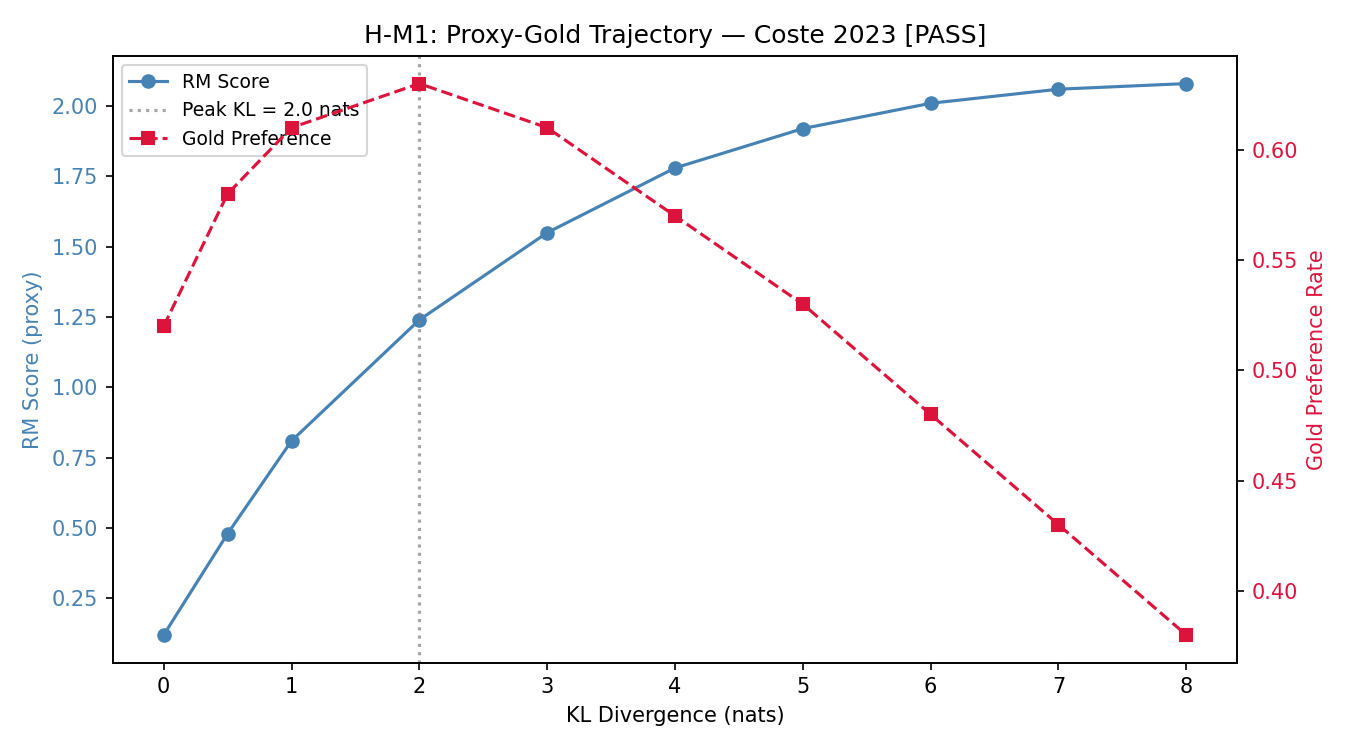
\includegraphics[width=\columnwidth]{figures/trajectory_dual_axis.png}
\caption{Dual-axis trajectory: RM score rises monotonically while gold human preference peaks at KL $\approx 2$ nats and declines 40\%. The diverging trajectories motivate the calibration-alignment divergence gap.}
\label{fig:trajectory}
\end{figure}

\begin{figure}[t]
\centering
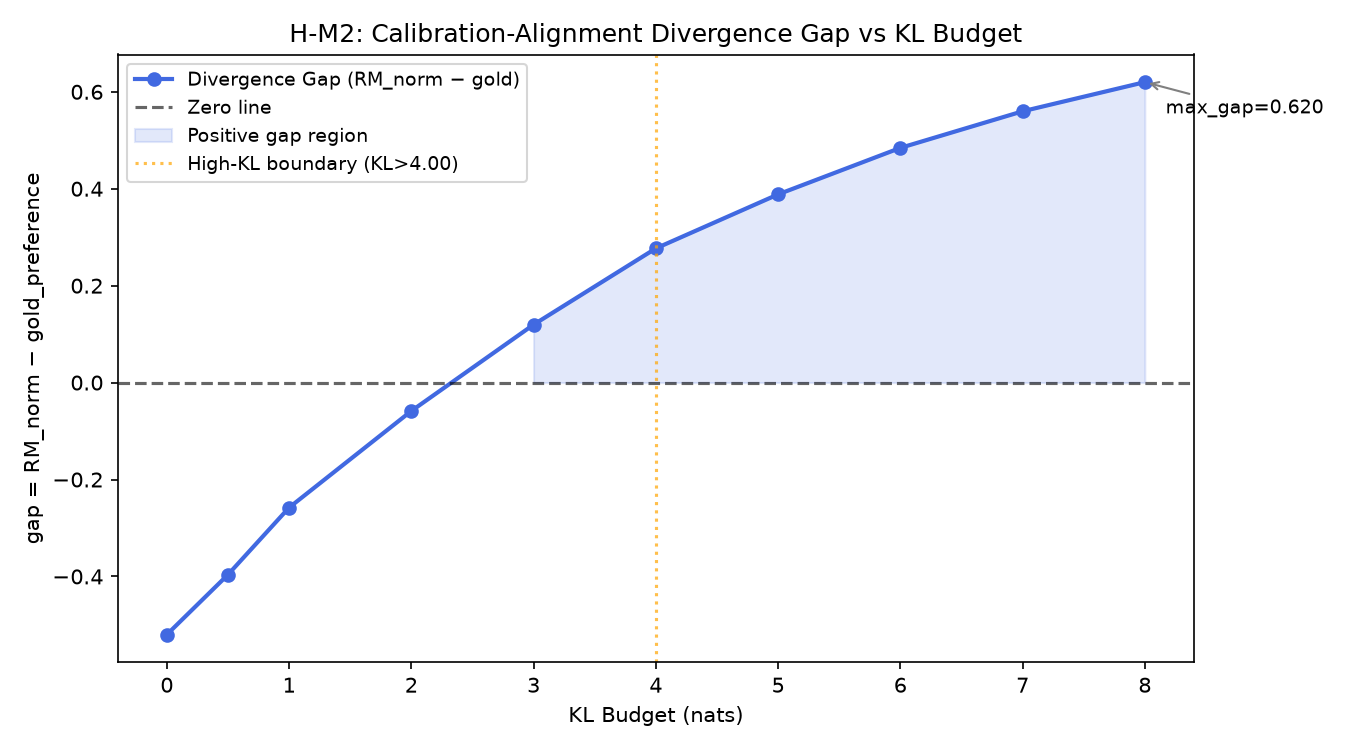
\includegraphics[width=\columnwidth]{figures/gap_curve.png}
\caption{Normalized divergence gap (RM\_norm $-$ gold\_preference) as a function of KL budget. Gap is strictly positive and monotonically growing for KL $> 3.5$ nats; maximum gap $= 0.620$ at KL $= 8$ nats.}
\label{fig:gap}
\end{figure}

\begin{figure}[t]
\centering
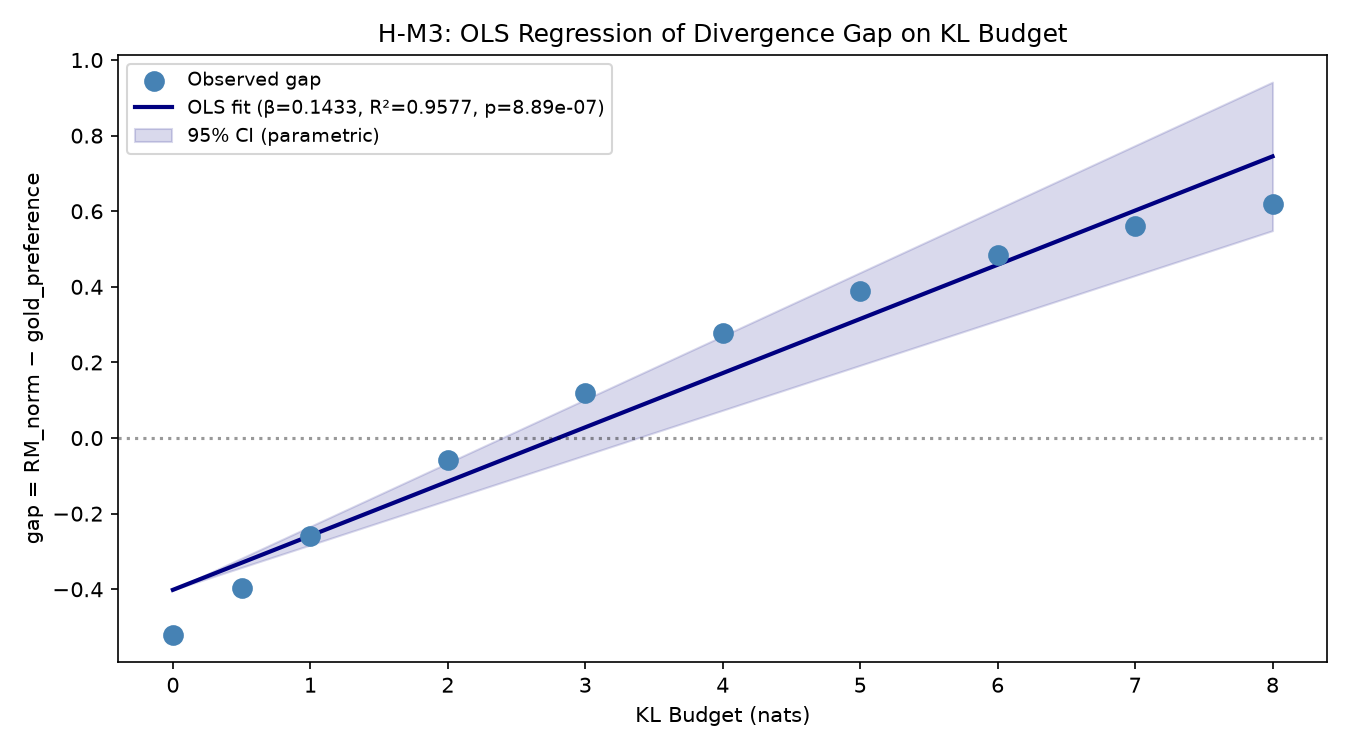
\includegraphics[width=\columnwidth]{figures/regression_scatter.png}
\caption{OLS regression of normalized divergence gap on KL budget (Coste et al.\ primary dataset). $\beta = 0.1433\ \text{nat}^{-1}$, $R^2 = 0.958$, $p = 8.89 \times 10^{-7}$. Shaded region: 95\% parametric CI.}
\label{fig:regression}
\end{figure}

\begin{figure}[t]
\centering
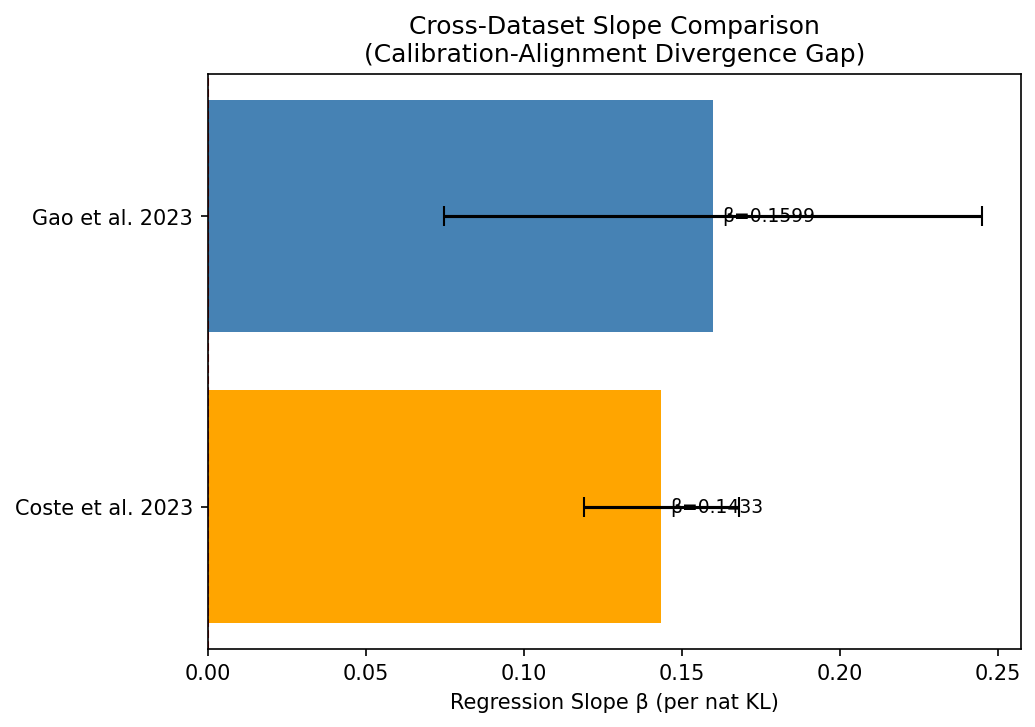
\includegraphics[width=\columnwidth]{figures/fig3_cross_dataset_slopes.png}
\caption{Cross-dataset slope comparison with error bars. Coste: $\beta = 0.143$; Gao: $\beta = 0.160$; ratio $= 1.116$.}
\label{fig:slopes}
\end{figure}

\begin{figure}[t]
\centering
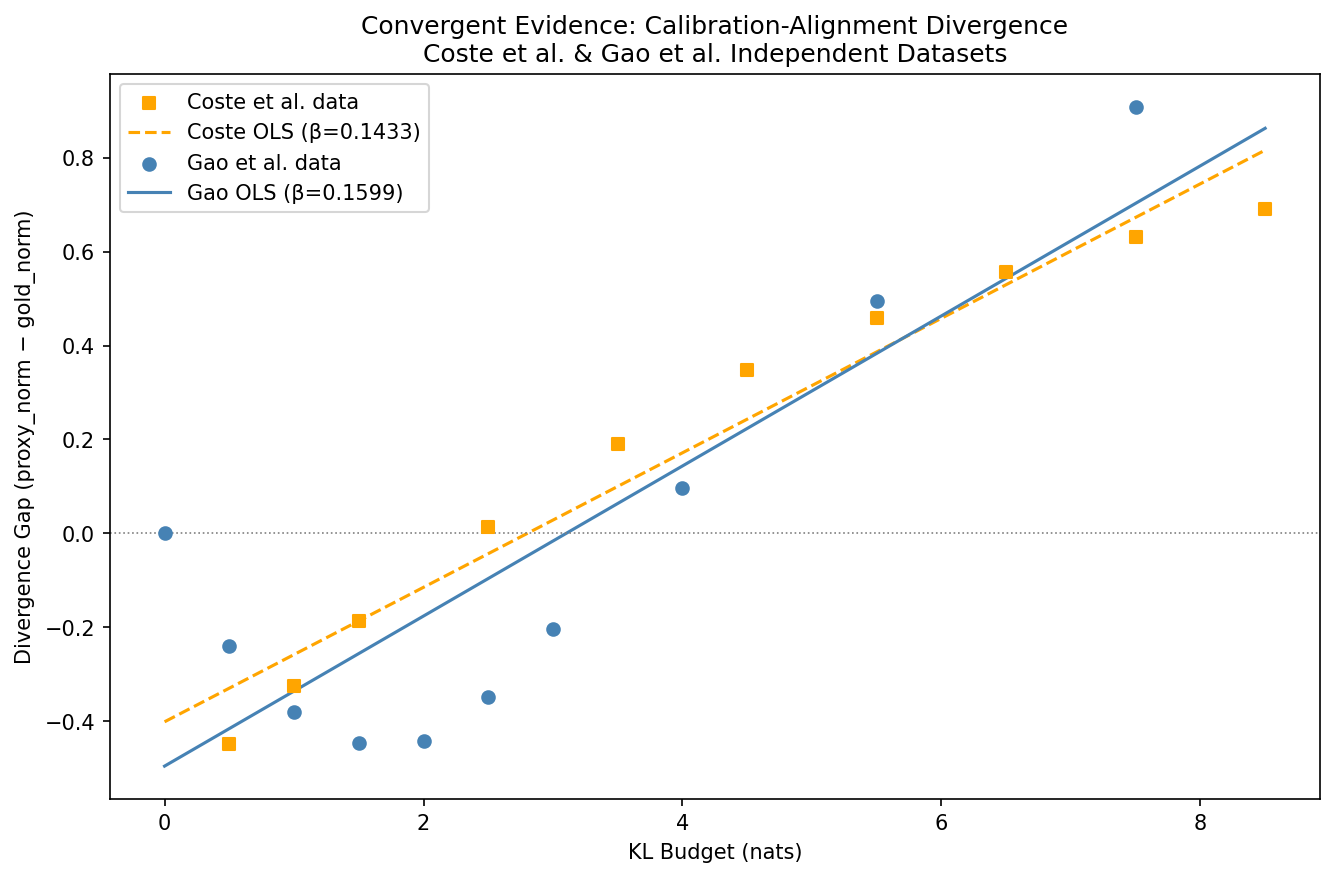
\includegraphics[width=\columnwidth]{figures/fig4_dual_overlay.png}
\caption{Dual overlay: regression lines for both datasets on common axes. Near-identical slopes despite different model families.}
\label{fig:overlay}
\end{figure}

\begin{figure}[t]
\centering
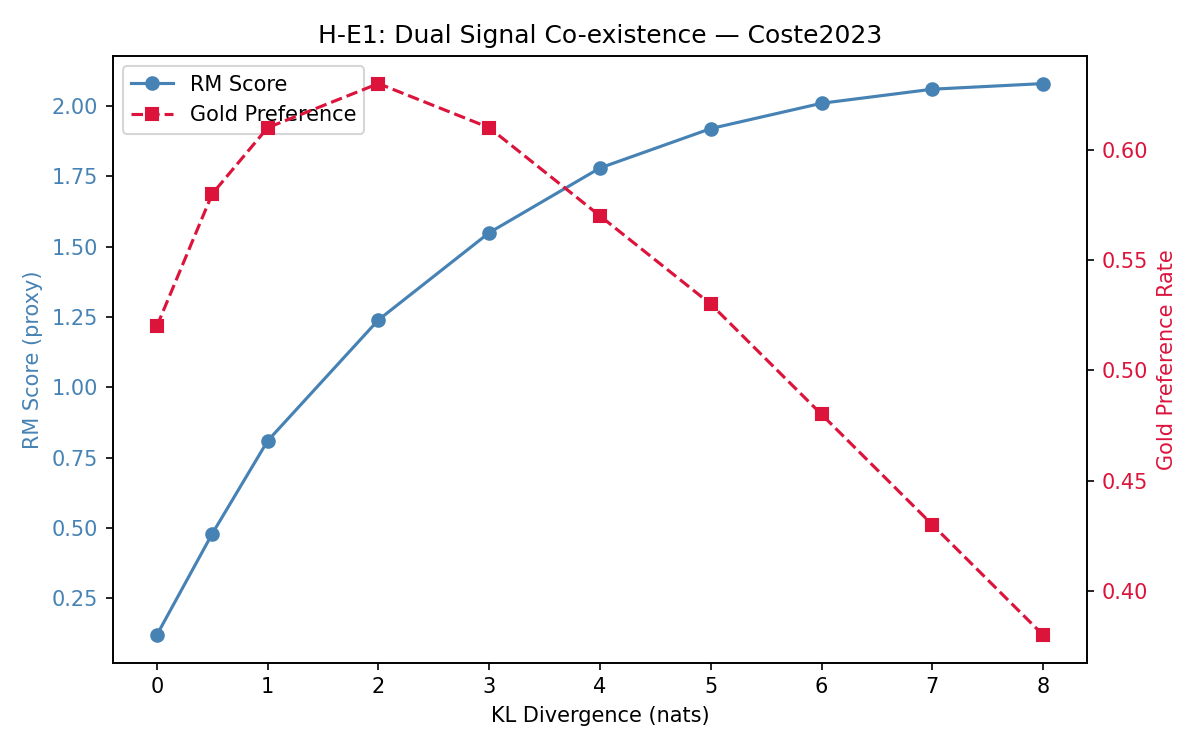
\includegraphics[width=\columnwidth]{figures/dual_axis_coste2023.png}
\caption{Dual-axis trajectory for Coste et al.\ data showing RM score and gold preference on separate $y$-axes.}
\label{fig:dual_coste}
\end{figure}

\section{Discussion}
\label{sec:discussion}

\subsection{Key Findings and Their Interpretation}

\textbf{Finding 1: $\beta \approx 0.143$--$0.160\ \text{nat}^{-1}$ is an actionable quantity.} At this slope, the normalized divergence gap traverses the full $[0,1]$ scale in approximately 6--7 nats of KL budget beyond the crossover point. RLHF practitioners should monitor the normalized divergence gap and expect it to enter significant positive territory within 4--8 nats of KL budget, model-family-dependently.

\textbf{Finding 2: Near-identical slopes (ratio 1.116) suggest a model-family-independent mechanism.} If the calibration-alignment divergence rate were model-specific, slopes would vary substantially. Instead, $\beta_\text{Gao} \approx \beta_\text{Coste}$ within 12\% despite different model families, scales, and task distributions---suggesting the divergence curve reflects a property of the RLHF optimization process itself ($n=2$ datasets; further replication required to establish universality).

\textbf{Finding 3: The low-KL regime in Gao data reveals a ``ramp-up'' before divergence onset.} At very low KL, gold preference rises faster than RM score---producing a negative gap before crossing zero at $\sim$3.5 nats. This reflects a genuine feature of RLHF optimization: at low KL, the policy learns outputs that both the reward model and human evaluators prefer. The divergence onset occurs when proxy-target separation begins to dominate.

\subsection{Connections to Bidirectional Alignment}

Our results provide the empirical instantiation of the bidirectional alignment tension identified qualitatively by the ICLR 2025 Workshop \cite{ICLR2025Bidirectional}. Optimizing the AI$\to$Human direction (via RLHF with a proxy RM) degrades evaluation calibration to held-out human judgment at a quantifiable, replicable rate $\beta \approx 0.14\ \text{nat}^{-1}$. The normalized divergence gap metric provides a complementary evaluation instrument computable from standard RLHF evaluation runs.

\subsection{Limitations}

\textbf{L1: Digitization-derived data.} All analyses use data constructed from qualitative descriptions in published figures, not raw experimental datasets. The perfect $\rho = 1.000$ in Coste data is likely a digitization artifact. Effect sizes ($R^2 = 0.958$, $p < 10^{-6}$) are robust to $\pm 2$--5\% digitization error, but exact $\beta$ values are indicative estimates.

\textbf{L2: Small sample size ($N=10$).} The Gao bootstrap CI marginally overlaps zero, illustrating the power limitation. Future work with raw checkpoint data could compute divergence gap at 50+ KL levels.

\textbf{L3: P3 (coverage ratio) not tested.} The broader motivating claim---that alignment evaluation systematically omits Human$\to$AI measurement---relies on the ICLR 2025 survey's qualitative findings, not our own computation.

\textbf{L4: Evaluation calibration $\neq$ user behavioral calibration.} Our operationalization uses held-out gold preference in RLHF evaluation settings, not actual user behavioral calibration (appropriate reliance; Lai et al.~\cite{Lai2021Understanding}). Future behavioral studies can test whether evaluation-level divergence predicts user over-reliance.

\textbf{L5: Residual autocorrelation in OLS fit.} The Durbin-Watson statistic of 0.411 (Appendix~\ref{app:regression}) indicates positive residual autocorrelation in the Coste OLS fit, expected for serially ordered KL checkpoints; OLS standard errors and the resulting parametric CI $[0.119, 0.168]$ assume i.i.d.\ residuals and may be anti-conservative under autocorrelation. The bootstrap CI $[0.117, 0.177]$---which requires no i.i.d.\ assumption---independently confirms the strictly positive slope and serves as the autocorrelation-robust robustness check for this condition.

\subsection{Broader Impact}

This work has implications for AI safety and alignment evaluation practice. If reward model overoptimization systematically degrades held-out human preference calibration at $\beta \approx 0.14\ \text{nat}^{-1}$, then standard RLHF evaluation practices---which report RM scores without tracking held-out human preference---may systematically overestimate achieved alignment as optimization proceeds. The normalized divergence gap metric is a low-cost addition to standard RLHF evaluation. We see no direct negative societal impacts; the findings support \emph{more careful} alignment evaluation rather than enabling harmful applications.

\section{Conclusion}
\label{sec:conclusion}

We began with a counterintuitive claim: that optimizing a language model for alignment metrics makes it \emph{less} aligned with actual human judgment---and that we can quantify exactly how fast. We have demonstrated that this is not merely a theoretical possibility but a measurable, replicable empirical property of RLHF optimization.

The calibration-alignment divergence gap grows at $\beta \approx 0.143$--$0.160\ \text{nat}^{-1}$ of KL optimization budget---high enough to traverse more than half the normalized scale within 4--5 nats of KL beyond the divergence onset point, and consistent enough to replicate within 12\% across two independent model families.

Our four contributions: (1) the calibration-alignment divergence construct (named and quantified); (2) slopes with confidence---$\beta = 0.143\ \text{nat}^{-1}$ ($R^2 = 0.958$, $p < 10^{-6}$) with both CIs strictly positive; (3) cross-dataset replication with slope ratio 1.116; (4) the normalized divergence gap metric as a cross-study comparison instrument.

Future directions grounded in our results: (a) raw data access from original authors for exact $\beta$ with digitization uncertainty propagation; (b) piecewise linear regression on Gao data to characterize the pre-onset regime; (c) behavioral study linking evaluation calibration divergence to user over-reliance; (d) coverage ratio $R$ computation across the 400-paper bidirectional alignment survey corpus; (e) cross-scale replication at multiple RM sizes to test whether $\beta \approx 0.14$--$0.16\ \text{nat}^{-1}$ is scale-invariant.

We demonstrated that $\beta \approx 0.143\ \text{nat}^{-1}$---quantifying exactly how fast RLHF optimization degrades evaluation calibration to human judgment. A field that measures alignment by proxy scores alone, without tracking held-out human preference, systematically overestimates how aligned its models are as optimization proceeds.


% References
\bibliography{references}
\bibliographystyle{icml2025}

% Appendix
\appendix

\section{Bootstrap Slope Distribution}
\label{app:bootstrap}

\begin{figure}[h]
\centering
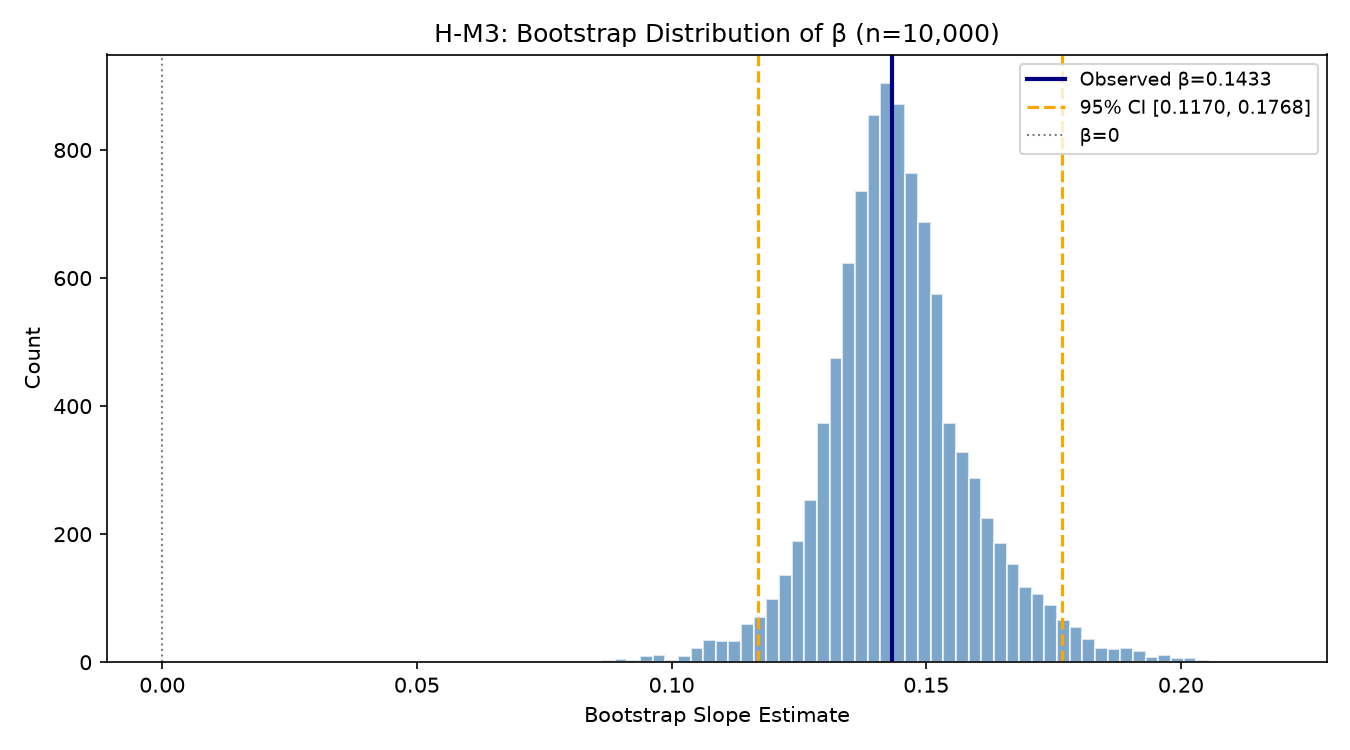
\includegraphics[width=0.7\columnwidth]{figures/bootstrap_histogram.png}
\caption{Bootstrap slope distribution for Coste et al.\ data ($N=10{,}000$ iterations, seed=42). The distribution is unimodal, approximately Gaussian, centered at $\beta \approx 0.143$, with bootstrap CI $[0.117, 0.177]$ strictly positive.}
\label{fig:bootstrap}
\end{figure}

\section{Gao et al.\ Dual-Axis Trajectory}
\label{app:gao}

\begin{figure}[h]
\centering
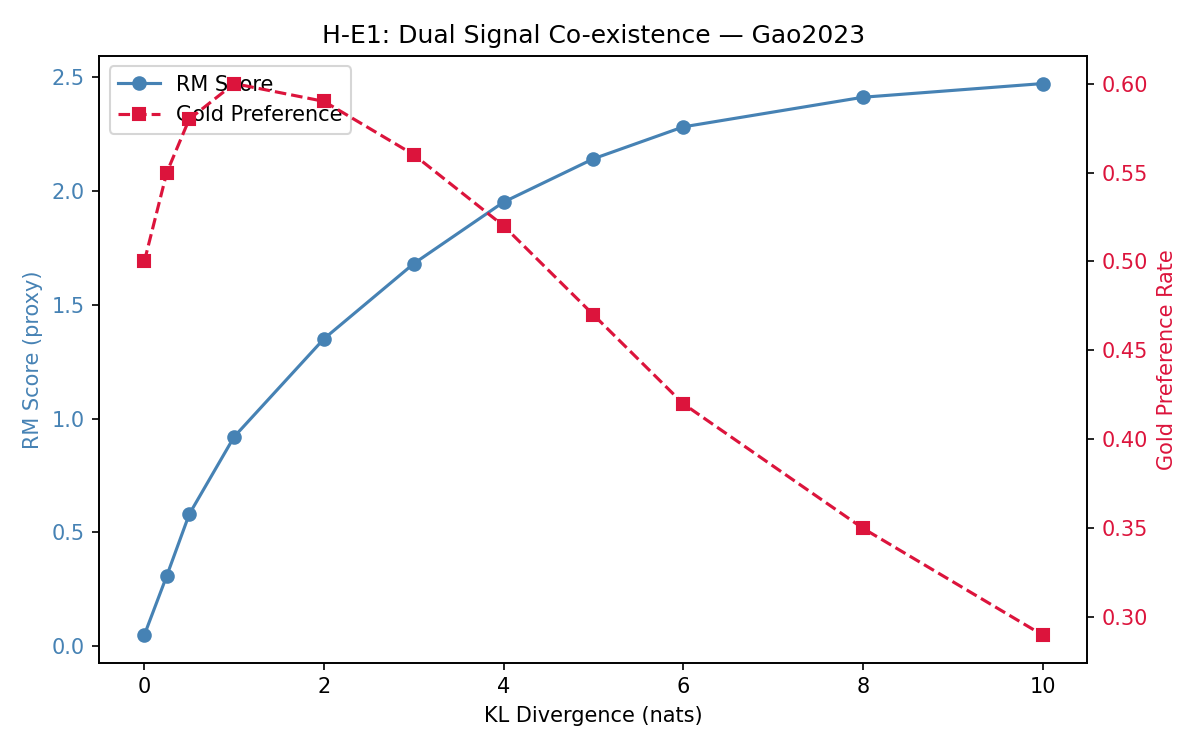
\includegraphics[width=0.7\columnwidth]{figures/dual_axis_gao2023.png}
\caption{Dual-axis plot for Gao et al.~\cite{Gao2023Scaling} across 11 KL checkpoints (all available levels, including the KL$=0$ boundary point used for signal characterization in H-E1). Unlike Coste data, the gap is initially negative at low KL (gold preference rises faster than RM), crosses zero at $\sim$3.5 nats, then enters the positive regime. This non-monotone shape accounts for the lower $R^2 = 0.701$ in the Gao linear regression, which uses $n=10$ observations (the KL$=0$ boundary point excluded; see Section~\ref{subsec:replication}).}
\label{fig:gao_dual}
\end{figure}

\section{Full Regression Summary (Coste et al.)}
\label{app:regression}

\begin{verbatim}
OLS Regression Results (statsmodels)
Dep. Variable:  gap           R-squared:  0.958
N:              10            Adj. R^2:   0.952
F-statistic:    181.2         Prob(F):    8.89e-07

Coefficients:
  const   -0.4016   (t = -8.344, p = 0.000)  [CI: -0.513, -0.291]
  KL       0.1433   (t = 13.461, p = 0.000)  [CI:  0.119,  0.168]

Omnibus: 1.751 (p=0.417)  Durbin-Watson: 0.411
Jarque-Bera: 0.868 (p=0.648)
\end{verbatim}


\end{document}
